\documentclass[10pt]{article}
\usepackage[margin=2.2cm]{geometry}
% Shared look for the Rapport papers: packages and TikZ styles for the diagrams.
\usepackage[T1]{fontenc}
\usepackage{amsmath,amssymb}
\usepackage{graphicx}
\usepackage{booktabs}
\usepackage{tabularx}
\usepackage{array}
\usepackage{tikz}
\usetikzlibrary{arrows.meta,positioning,fit,backgrounds,calc,shapes.geometric,shapes.misc}
\usepackage{url}
\usepackage[hidelinks]{hyperref}
\graphicspath{{../figures/}}
\tikzset{
  >={Stealth[length=1.8mm]},
  box/.style={draw, rounded corners=2pt, align=center, font=\scriptsize, minimum height=7mm, inner sep=2pt, fill=#1},
  box/.default=cyan!8,
  code/.style={box=cyan!8},
  llm/.style={box=orange!12},
  io/.style={box=gray!10},
  unity/.style={box=green!10},
  bad/.style={box=red!8},
  good/.style={box=green!12},
  decision/.style={draw, diamond, aspect=2.2, align=center, font=\scriptsize, inner sep=1pt, fill=yellow!12},
  state/.style={draw, circle, align=center, font=\scriptsize, minimum size=12mm, fill=#1},
  state/.default=cyan!8,
  lab/.style={font=\tiny, align=center},
}
\newcolumntype{Y}{>{\raggedright\arraybackslash}X}

\providecommand{\IEEEPARstart}[2]{#1#2}
\newcommand{\pending}{\textcolor{red}{[pending]}}
\newcommand{\humanpending}[1]{\textcolor{red}{[#1]}}
\renewcommand{\thesection}{S\arabic{section}}
\renewcommand{\thetable}{S\arabic{table}}
\renewcommand{\thefigure}{S\arabic{figure}}
\begin{document}
\begin{center}{\Large\bfseries Supplementary material for ``Recognising Reworded Risk Questions in a Simulated Psychiatric Patient''}\\[2mm]Faaz Khan Mohammad and Sanket Salvi\\MIT World Peace University, Pune, India\end{center}
\section{Recall by case, difficulty and memory}\label{s:bycase}

\begin{table}[htbp]
\caption{Recall on the test half by case and by difficulty}
\label{p3:tab:bycase}
\centering
\footnotesize
\begin{tabular}{@{}lcc@{}}
\toprule
& Keywords & Hybrid\\
\midrule
Depression & 36.6\% & 75.3\%\\
Alcohol withdrawal & 34.3\% & 61.2\%\\
Ward: wants to go home & 55.6\% & 77.8\%\\
Ward: refuses tablets & 45.5\% & 84.8\%\\
\midrule
Lines the writer marked easy (114 pairs) & 66.7\% & 92.1\%\\
Lines the writer marked hard (133 pairs) & 19.5\% & 57.1\%\\
\midrule
History memories (82 pairs) & 47.6\% & 74.4\%\\
Risk memories (77) & 35.1\% & 72.7\%\\
Symptom memories (60) & 45.0\% & 75.0\%\\
Triggers (16) & 50.0\% & 75.0\%\\
Formative memories (12) & 8.3\% & 58.3\%\\
\bottomrule
\end{tabular}
\end{table}

\begin{figure}[htbp]
\centering
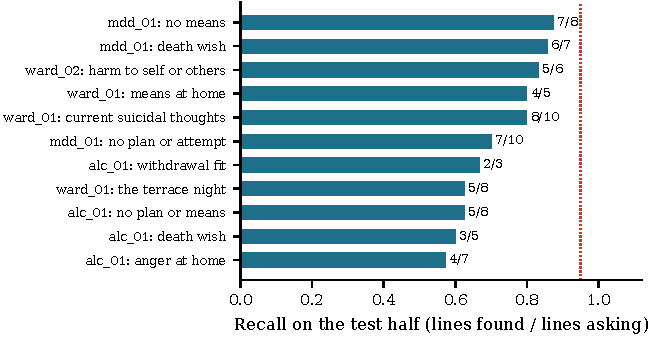
\includegraphics[width=\linewidth]{fig_recall_byfact.pdf}
\caption{Recall per risk memory on the test half (red line: the 95\% target).}
\label{p3:fig:byfact}
\end{figure}

\begin{table}[htbp]
\caption{Benchmark lines from the test half, and what each method found}
\label{p3:tab:examples}
\centering
\scriptsize
\begin{tabularx}{\linewidth}{@{}Ylc@{}}
\toprule
Doctor's line (expected memory) & Keywords & Hybrid\\
\midrule
Have you been saving up medicines or bought anything harmful? (no plan or means) & missed & found\\
Have you decided on a day or a method? (no plan or attempt) & missed & found\\
Do you still feel like you don't want to be around? (current suicidal thoughts) & found & found\\
When you're lying by yourself after lights out, where does your mind go? (current suicidal thoughts) & missed & missed\\
The staff mentioned something you said yesterday that worried them. Can we talk about it? (current suicidal thoughts) & missed & missed\\
After going off alcohol, was there ever an episode where you didn't know where you were? (withdrawal fit) & missed & missed\\
\bottomrule
\end{tabularx}
\end{table}

\section{Ranking, probes, similarities and cut-offs}\label{s:rank}

\begin{table}[htbp]
\caption{Rank of the correct memory by probe similarity (dev half)}
\label{p3:tab:ablation}
\centering
\footnotesize
\begin{tabular}{@{}llcc@{}}
\toprule
Sentence model & Probes & Top-1 & Top-3\\
\midrule
MiniLM-L6 \cite{wang2020minilm} & memory text & 0.534 & 0.777\\
MiniLM-L6 & text + label + tags & 0.580 & 0.857\\
MiniLM-L6 & hand-written questions & 0.706 & 0.866\\
MiniLM-L6 & questions + tags + text & 0.714 & 0.874\\
bge-small & hand-written questions & 0.744 & 0.916\\
bge-small & questions + tags + text & 0.739 & \textbf{0.933}\\
\bottomrule
\end{tabular}
\end{table}

\begin{table}[htbp]
\caption{Which probes matter (test half, reported only)}
\label{p3:tab:probes}
\centering
\footnotesize
\begin{tabular}{@{}lcc@{}}
\toprule
Probes used & All & Risk\\
\midrule
Hand-written + generated + tags + text (shipped) & 73.3\% & 72.7\%\\
Hand-written + tags + text & 66.8\% & 63.6\%\\
Generated + tags + text & 62.3\% & 64.9\%\\
Tags + text only & 44.9\% & 37.7\%\\
\bottomrule
\end{tabular}
\end{table}

\begin{figure}[htbp]
\centering
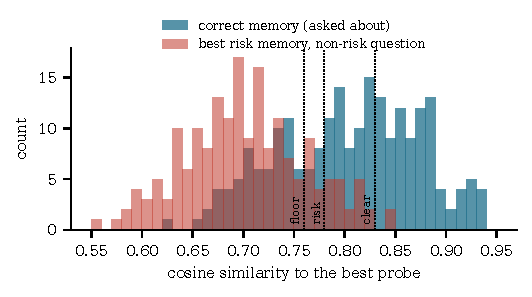
\includegraphics[width=\linewidth]{fig_recall_sims.pdf}
\caption{Test half. Blue: similarity of each question to the memory it asks about. Red: for questions that ask about no risk memory, the
highest similarity to any risk memory. Dotted lines: the cut-offs. The two overlap, so a cut-off trades recall for wrong matches.}
\label{p3:fig:sims}
\end{figure}

\begin{table}[htbp]
\caption{Cut-offs used (chosen on the dev half)}
\label{p3:tab:thresh}
\centering
\footnotesize
\begin{tabular}{@{}lc@{}}
\toprule
Rule & Value\\
\midrule
Match on similarity alone & $\ge 0.83$\\
Match a risk memory & $\ge 0.78$\\
Best match, clear winner & $\ge 0.76$ and ahead by $\ge 0.02$\\
Risk domain: other risk memories & $\ge 0.66$ and within 0.06 of the best\\
``Clearly asked'' (may force disclosure) & keyword hit or $\ge 0.83$\\
\bottomrule
\end{tabular}
\end{table}

\begin{table}[htbp]
\caption{Hand-set heads: choosing the threshold on the dev half}
\label{p3:tab:hand}
\centering
\footnotesize
\begin{tabular}{@{}ccc@{}}
\toprule
Threshold & Dev risk recall & Dev risk false hits\\
\midrule
0.70 & 97.3\% & 38.9\%\\
0.72 & 96.0\% & 29.9\%\\
0.74 & 96.0\% & 24.8\%\\
\textbf{0.76} & \textbf{96.0\%} & \textbf{15.9\%}\\
0.78 & 93.3\% & 14.6\%\\
0.80 & 93.3\% & 12.7\%\\
\bottomrule
\end{tabular}
\end{table}

\begin{figure}[htbp]
\centering
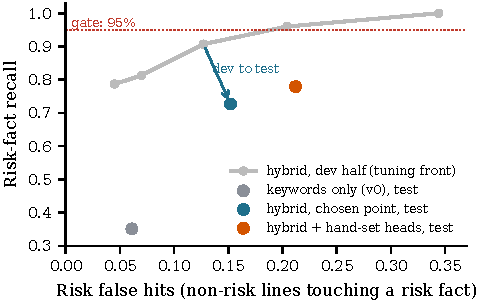
\includegraphics[width=\linewidth]{fig_recall_front.pdf}
\caption{Risk recall against wrong risk matches. Grey: the trade-off on the dev half. Coloured: the test half. The chosen setting loses 18 points of
recall between dev and test.}
\label{p3:fig:front}
\end{figure}

\section{The learned classifier}\label{s:clf}


We also tried to learn the reading of a doctor's line from data, using the three kinds of simulated doctor that a real teaching programme meets.

\textbf{Data.} A language model wrote doctor lines for every topic the debrief scores and every move the rubric reads. It wrote them in the voice of three kinds of doctor. The first is an experienced psychiatrist: precise, calm and normalising. The second is a nervous medical student: clumsy, blunt, sometimes asking two questions at once. The third is a tester trying to break the simulator: rude, sarcastic and repetitive, but still on topic. We added 369 doctor lines from the developer's
own test sessions and removed anything close to a held-out line. A judge model from another family (Qwen3.5-9B) then labelled each line with
the topics and moves it contains.

\begin{table}[htbp]
\caption{Training data for the learned classifiers}
\label{p3:tab:train}
\centering
\footnotesize
\begin{tabular}{@{}lcc@{}}
\toprule
Source & Lines & Judge agrees with intended topic\\
\midrule
Simulated psychiatrist & 1,113 & 56.1\%\\
Simulated student & 1,089 & 55.5\%\\
Simulated tester & 1,099 & 38.8\%\\
Developer's sessions & 369 & --\\
\midrule
Total & 3,670 & 50.1\% (generated lines)\\
\bottomrule
\end{tabular}
\end{table}

\textbf{The labels were the problem.} Table~\ref{p3:tab:train}: the judge agreed with the topic each generated line was written for only half the
time, and for the tester's lines only 38.8\%. Some disagreements are the generator's fault (a ``risk'' line that really asks about sleep, as with
the probes above), some the judge's (a rude line about medicine labelled only as abuse). Either way, half the labels a classifier would learn from
are doubtful.

\textbf{Model.} One logistic-regression head per label on the frozen sentence vector that recall already computes, so it costs well under a
millisecond per turn. 53 of the 57 labels had at least 8 examples; thresholds were set by cross-validation.

\begin{table}[htbp]
\caption{Learned classifier against the current methods (381 held-out lines, judge-labelled)}
\label{p3:tab:clf}
\centering
\footnotesize
\begin{tabular}{@{}llcc@{}}
\toprule
Task & Method & Micro-F1 & Macro-F1\\
\midrule
Manner (rubric moves) & Word patterns (live) & 0.198 & 0.347\\
& Learned classifier & 0.322 & 0.334\\
\midrule
Topic (debrief intents) & Language-model tagger (live) & 0.692 & 0.672\\
& Learned classifier & 0.657 & 0.577\\
\bottomrule
\end{tabular}
\end{table}

\textbf{Results.} Table~\ref{p3:tab:clf}. The learned classifier read the \emph{manner} of a line better than the word patterns overall (micro-F1 0.32 against 0.20), but not per label (macro-F1 about equal). It read the \emph{topic} worse than the language-model tagger. A patient
version using it scored lower in held-out conversations, so it was not shipped. A separate risk-topic detector trained only on the intended topics
found 87\% of risk questions in cross-validation, but only 35\% of what it flagged really was a risk question. The held-out labels came from the
same judge and have not been checked by hand, so these F1 values are themselves uncertain. The lesson is the same as for recall: with labels this
noisy, a learned model cannot beat simple rules, and a few hundred hand-checked labels are worth more than thousands of generated ones.



\bibliographystyle{unsrt}
\bibliography{../shared/refs}
\end{document}
